
\section{Färbungen}
	\authors{Josua Kugler und Amelie Koch}
	
	Ein Teilgebiet der Graphentheorie, nämlich die Färbung von Graphen, bietet Raum für zahlreiche Anwendungen. Im Folgenden möchten wir ein solches Anwendungsbeispiel näher betrachten.
	\subsection{Knotenfärbung}
	\begin{table*}
	\centering
	\begin{tabular}{c|c|c|c|c|c|c}
		Zahlentheorie& Robotik & Astronomie & Ökologie & Wirtschaft & Biologie & Chemie\\\hline
		$T_1$&$T_3$ &$T_3$ & $T_5$ & $T_6$ & $T_6$ & $T_6$\\
		$T_2$&$T_4$ &$T_5$ &   &   &   & $T_5$\\
		& $T_1$ & $T_4$ &   &   &   & $T_4$\\
		& $T_2$ & $T_2$ &   &   &   & $T_1$\\	
	\end{tabular}
	\caption{Kurswahl von 6 TeilnehmerInnen $T_1$ bis $T_6$}
	\label{kurswahlen}
	\end{table*}

\begin{figure}
\centering
	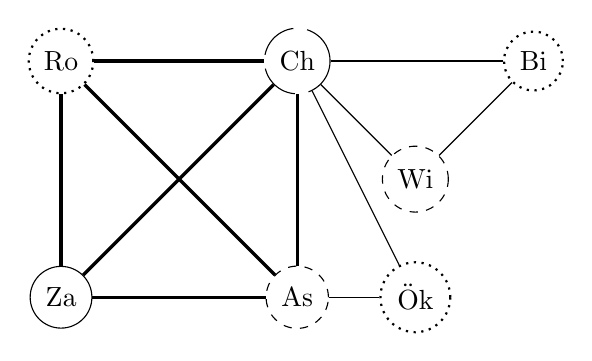
\begin{tikzpicture}[scale=0.5]
	\node[draw,circle,dashed](As) at (6,0){As};
	\node[draw,circle,dotted,thick](Ro) at (0,6){Ro};
	\node[draw,circle](Za) at (0,0){Za};
	\node[draw,circle,dotted,thick](Ök) at (9,0){Ök};
	\node[draw,circle,dashed](Wi) at (9,3){Wi};
	\node[draw,circle,dotted,thick](Bi) at (12,6){Bi};
	\node[draw,circle,dash pattern=on 15pt off 5pt](Ch) at (6,6){Ch};
	\draw[very thick] (Ro)--(As);
	\draw[very thick] (Za)--(Ro);
	\draw[very thick] (Ro)--(Ch);
	\draw[very thick] (As)--(Ch);
	\draw[very thick] (Za)--(Ro);
	\draw[very thick] (Za)--(Ch);
	\draw[very thick] (Za)--(As);
	\draw (As)--(Ök);
	\draw(Ök)--(Ch);
	\draw(Wi)--(Bi);
	\draw(Bi)--(Ch);
	\draw(Wi)--(Ch);
	\end{tikzpicture}	
\caption{Dies ist der Graph, der die Kurswahlen aus Tabelle \ref{kurswahlen} darstellt. Kurse werden als Knoten dargestellt, die Konflikte zwischen Kursen als Kanten. Die Farben werden durch  verschiedene Knotenumrandungen repräsentiert.}
\label{problem1}
\end{figure}
	Angenommen, die DSA kann im Jahr 2028 allen Teilnehmern ermöglichen, alle gewählten Kurse zu besuchen. 
	Wie viele Akademien müssen bei einer Kurswahl wie in Tabelle \ref{kurswahlen} mindestens stattfinden, wenn alle TeilnehmerInnen nur einen Kurs pro Akademie besuchen können?

	Für die geringste Zahl an Akademien muss versucht werden, möglichst viele TeilnehmerInnen auf einer Akademie unterzubringen. Wie können wir an dieses Problem herangehen?
Hier hilft ein graphentheoretischer Ansatz weiter. Hierfür wählen wir die Kurse als Knoten.  Kurse, die nicht gleichzeitig stattfinden dürfen, da sie beide von der gleichen Person gewählt wurden, werden durch eine Kante verbunden. Diese Kurse stehen in Konflikt miteinander, sie müssen also auf verschiedenen Akademien stattfinden.
Wir wissen also, dass benachbarte Knoten auf unterschiedlichen Akademien stattfinden müssen. Dies können wir veranschaulichen, indem benachbarte Knoten unterschiedlich eingefärbt werden. Jede Akademie wird dann durch eine andere Farbe repräsentiert. Wie in Abb. \ref{problem1} zu erkennen, benötigt man in unserem Beispiel
 höchstens vier Farben bzw. Akademien. Kann diese Zahl verringert werden?
Dass dies nicht möglich ist, erkennt man an den Kanten zwischen Robotik, Chemie, Zahlentheorie und Astronomie im Graphen (fett hervorgehobene Kanten in Abb. \ref{problem1}). Diese Knoten sind vollständig miteinander verbunden, sodass sie verschieden eingefärbt sein müssen.


	\begin{df}
		Eine \wichtig{$k$-Färbung} eines Graphen $G=(V,E)$ ist eine Funktion $c:\ V\to\{1,2,\dots,k\}$, sodass für jede Kante $e=\{v_1,v_2\}$ gilt: $c(v_1)\neq c(v_2)$.\\
Ein Graph heißt \wichtig{$k$-färbbar}, wenn eine $k$-Färbung des Graphen existiert.
	\end{df}
	\begin{df}
		Die \wichtig{chromatische Zahl $\chi(G)$} eines Graphen $G=(V,E)$ 
 ist das kleinste $k$, sodass $G$ $k$-färbbar ist.
	\end{df}
	\subsection{Kantenfärbung}
	Die DSA bietet im Jahr 2038 allen TeilnehmerInnen Einzelunterricht an. Auf einer Akademie wird jeder Kurs weiterhin höchstens einmal angeboten und alle TeilnehmerInnen belegen jeden gewählten Kurs genau einmal. Jeder Kurs wird auf mehreren Akademien angeboten und jeder Teilnehmer und jede Teilnehmerin besucht auf einer Akademie genau einen Kurs.
 Wie viele Akademien werden nun bei den Kurswahlen aus Tabelle \ref{kurswahlen}  benötigt?
\begin{figure}
\centering
	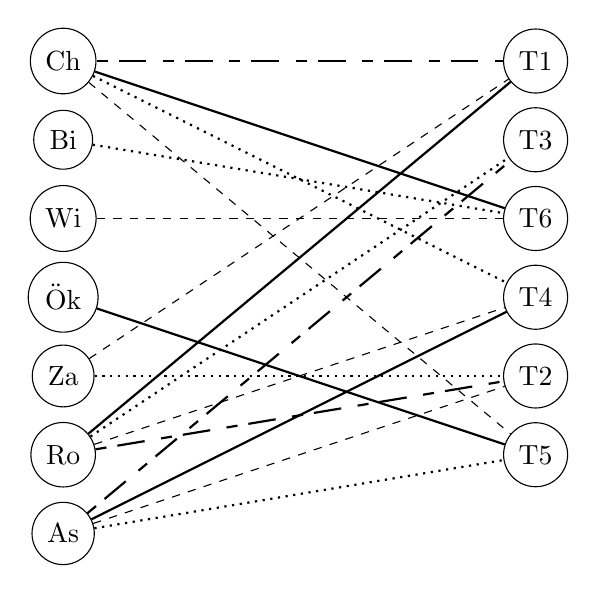
\begin{tikzpicture}
	%Kurse
	\node[draw,circle](As) at (0,0){As};
	\node[draw,circle](Ro) at (0,1){Ro};
	\node[draw,circle](Za) at (0,2){Za};
	\node[draw,circle](Ök) at (0,3){Ök};
	\node[draw,circle](Wi) at (0,4){Wi};
	\node[draw,circle](Bi) at (0,5){Bi};
	\node[draw,circle](Ch) at (0,6){Ch};
	%Schüler
	\node[draw,circle](A) at (6,1){T5};
	\node[draw,circle](C) at (6,2){T2};
	\node[draw,circle](J) at (6,3){T4};
	\node[draw,circle](N) at (6,4){T6};
	\node[draw,circle](P) at (6,5){T3};
	\node[draw,circle](T1) at (6,6){T1};
	%Kurswahlen
	\draw[dashed] (Za)--(T1);
	\draw[thick,dotted] (Za)--(C);
	\draw[thick,dotted] (Ro)--(P);
	\draw[thick,dash pattern=on 4pt off 4pt on 10pt off 6pt] (Ro)--(C);
	\draw[dashed](Ro)--(J);
	\draw[thick](Ro)--(T1);
	\draw[thick,dash pattern=on 4pt off 4pt on 10pt off 6pt] (As)--(P);
	\draw[thick](As)--(J);
	\draw[thick,dotted] (As)--(A);
	\draw[dashed] (As)--(C);
	\draw[thick](Ök)--(A);
	\draw[dashed] (Wi)--(N);
	\draw[thick,dotted] (Bi)--(N);
	\draw[thick](Ch)--(N);
	\draw[dashed] (Ch)--(A);
	\draw[thick,dotted] (Ch)--(J);
	\draw[thick,dash pattern=on 4pt off 4pt on 10pt off 6pt] (Ch)--(T1);
	\end{tikzpicture}
\caption{Kurse werden durch die Knoten auf der linken Seite dargestellt, TeilnehmerInnen auf der rechten Seite, Kanten stellen die Belegungen dar, unterschiedliche Kantenfärbungen entsprechen der Art der Linie.}
\label{problem2}
\end{figure}

Das Problem liegt hier darin begründet,  die von den  TeilnehmerInnen gewählten Kurse so auf unterschiedliche Akademien zu verteilen, dass insgesamt möglichst wenige Akademien stattfinden müssen.
Auch dieses Verteilungsproblem lässt sich mathematisch mittels eines Graphen beschreiben.
Allerdings müssen jetzt nicht mehr nur die Kurse, sondern auch TeilnehmerInnen auf Akademien verteilt werden.
Wir müssen also stets Paare (Kurs, Teilnehmer) einzelnen Akademien zuordnen.
Wie kann dies im Graph dargestellt werden?

Das Tupel  (Kurs, Teilnehmer) entspricht in einem Graphen der Kante zwischen dem Knoten \glqq Kurs \grqq\ und dem Knoten \glqq Teilnehmer\grqq. Diese Knoten werden dann entsprechend ihrer Belegungen verbunden. Welche dieser Tupel dürfen nicht zusammen auf einer Akademie vorkommen? Stimmen TeilnehmerIn oder Kurs (also ein Knoten) zweier solcher Tupel überein, so können diese nicht beide auf einer Akademie sein.  Kennzeichnet man nun wie oben unterschiedliche Akademien mit unterschiedlichen Farben, ergibt sich folgende Regel für die Färbung: Zwei Kanten, die mit dem gleichen Knoten verbunden sind, dürfen nicht die gleiche Farbe haben. 
So kann über eine Kantenfärbung (oder äquivalent eine Knotenfärbung des Liniengraphen)  eine Lösung für das Problem gefunden werden. Wie in Abb. \ref{problem2} zu erkennen ist, reichen auch in diesem Fall vier Farben aus. Dieser Graph kann nicht mit weniger Farben gefärbt werden, da es Knoten mit Grad vier gibt.
	\begin{df}
		Eine \wichtig{$k$-Kantenfärbung} eines Graphen $G=(V,E)$ ist eine Funktion $c : E \to \{1,\dots,k\}$, sodass für jeden Knoten $v$ gilt:
		Für alle $e_1,e_2\in E$ mit $e_1\neq e_2$ und $v\in e_1,v\in e_2$ gilt $c(e_1)\neq c(e_2)$.\\
		Ein Graph heißt \wichtig{$k$-kantenfärbbar}, wenn eine $k$-Kantenfärbung des Graphen existiert.
	\end{df}
	\begin{df}
Das kleinste $k$, für das ein Graph $G$ $k$-kantenfärbbar ist, heißt \wichtig{chromatischer Index $\chi'(G)$}.
	\end{df}



\subsection{Schranken für $\chi(G)$ und $\chi '(G)$} 
\begin{figure}
\centering
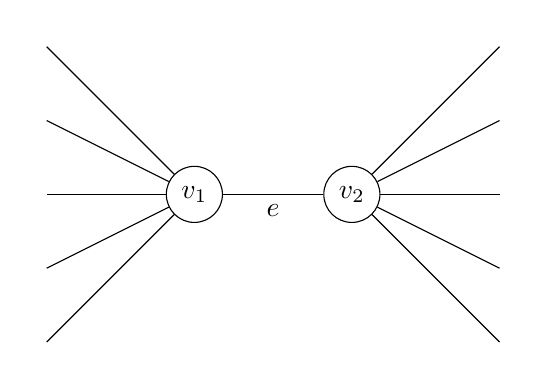
\begin{tikzpicture}
\node[circle,draw] (1) at (-1,0){$v_1$};
\node[circle,draw] (2) at (1,0){$v_2$};
\node (11) at (-3,-2){};
\node (12) at (-3,-1){};
\node (13) at (-3,0){};
\node (14) at (-3,1){};
\node (15) at (-3,2){};
\node (21) at (3,-2){};
\node (22) at (3,-1){};
\node (23) at (3,0){};
\node (24) at (3,1){};
\node (25) at (3,2){};



\draw (1)--node[below] {$e$}(2);
\draw (1)--(11);
\draw (1)--(12);
\draw (1)--(13);
\draw (1)--(14);
\draw (1)--(15);
\draw (2)--(21);
\draw (2)--(22);
\draw (2)--(23);
\draw (2)--(24);
\draw (2)--(25);


\end{tikzpicture}
\caption{Obere Schranke für $\chi'(G)$?}
\label{chi_oben}
\end{figure}
Es stellt sich nun die Frage, ob man die chromatische Zahl bzw. den chromatischen Index abschätzen
 kann, wenn man den Maximalgrad $\Delta$ eines Graphen kennt. 
Eine untere Schranke für $\chi'(G)$ ist bereits dadurch gegeben, dass bei einem Knoten mit dem Maximalgrad $\Delta$ genau $\Delta$ Kanten zusammenlaufen, man benötigt also mindestens $\Delta$ Farben für eine Kantenfärbung.

Um eine Kantenfärbung zu bestimmen, kann man nach folgendem Greedy-Algorithmus vorgehen: Um die Farbe einer Kante $e=\{v_1,v_2\}$ zu bestimmen, betrachtet man die Farben aller angrenzenden Kanten $e_i$ mit $v_1\in e_i\lor v_2\in e_i$ und färbt die Kante $e$ mit einer Farbe, die nicht für eine der Kanten $e_i$ verwendet wurde.
Eine obere Schranke kann man zunächst einmal dadurch bestimmen, dass man den Worst Case
betrachtet: Eine Kante $e$, deren Knoten $v_1$ und $v_2$ jeweils den Maximalgrad besitzen (siehe Abb. \ref{chi_oben} mit $\Delta=6$). Sollten alle Kanten unterschiedlich gefärbt sein  (es sei dahingestellt, ob das tatsächlich auch möglich ist), so kommt man mithilfe des Greedy-Algorithmus auf $2\Delta-2$ zu $e$ \glqq benachbarte\grqq\  Kanten und damit $2\Delta-1$ Farben.
Diese obere Schranke lässt sich aber noch weiter herabsetzen.
\begin{satz}[Vizing]
 $\Delta\leq\chi'(G)\leq\Delta+1$
\end{satz}
Ähnliches lässt sich auch für die chromatische Zahl feststellen. Wenn man von $|V|\leq1$ absieht, beträgt hier die untere Schranke $2$.
Das liegt daran, dass bipartite Graphen mit beliebigem Maximalgrad mit zwei Farben gefärbt werden können. Für vollständige Graphen erhält man bereits $\Delta+1$ benötigte Farben, da jeder Knoten mit $\Delta$ anderen Knoten verbunden ist und es daher nicht möglich ist, eine Farbe zweimal zu verwenden. Zu zeigen  bleibt, dass es keine Graphen gibt, die eine größere Anzahl an Farben benötigen.
 Folgender nicht leicht zu beweisender Satz bestätigt unsere Vermutung.
\begin{satz}[Brooks]
 $\chi(G)\leq\Delta+1$ und die einzigen zusammenhängenden Graphen mit $\chi(G)=\Delta+1$ sind die vollständigen Graphen und Kreise mit ungerader Anzahl an Knoten. 
\end{satz}
Ein mögliches Anwendungsbeispiel ist die Organisation eines Schachturniers mit $n$ TeilnehmerInnen. Wie viele Runden müssen mindestens gespielt werden, damit jeder gegen jeden spielt? Auch dieses Problem lässt sich mithilfe eines Graphen modellieren. Die TeilnehmerInnen werden als Knoten dargestellt, ein Spiel als Kante zwischen den Gegnern. Die Lösung des Problems besteht in einer Kantenfärbung, wobei eine Farbe einer Runde entspricht. Nach dem Satz von Vizing müssen höchstens $\Delta+1$, also in unserem Fall $(n-1)+1=n$ Runden gespielt werden.